\chapter{脊髓中的感觉-运动整合} \label{chap:chap32}

在有目的的运动中,中枢神经系统使用大量来自感觉受体的信息来确保肌肉活动的模式适合目的。
没有这种感官信息,动作往往不精确,需要双手精细协调的任务(例如扣衬衫扣子)就很困难。
使运动的持续调节成为可能的感觉运动整合发生在神经系统的许多层面,但脊髓具有特殊的作用,因为脊髓中感觉输入和运动输出到肌肉之间的紧密耦合。


\textit{查尔斯$\cdot$谢林顿}是最早认识到感官信息在调节运动中重要性的人之一。
1906 年,他提出简单的反射(由皮肤或肌肉中的感受器激活引起的刻板运动)是运动的基本单位。
他还强调,神经系统的所有部分都是相互联系的,没有任何部分能够在不影响或受其他部分影响的情况下激活。
用他的话说,简单的反射即使不是一种可能的虚构,也是一种方便的。


从 1950 年代及以后对动物反射的实验室研究表明,下行运动通路和传入感觉通路会聚在脊髓中共同的中间神经元上。
后来对完整动物和从事正常行为的人类的研究证实,脊髓中的神经回路通过整合下行运动指令和感觉反馈信号,参与向肌肉传递和塑造运动指令。
然而,简单反射的概念有助于理解脊髓中感觉运动整合的组织原理,以及不同脊髓回路的感觉输入如何促进运动控制。


在本章中,我们解释了脊髓中感觉-运动整合的基本原理,并描述了这种整合如何调节运动。
为此,我们必须首先全面了解脊髓中的反射通路是如何组织的。



\section{脊髓中的反射通路产生肌肉收缩的协调模式}

激活脊髓反射通路的感觉刺激在脊髓外作用于肌肉、关节和皮肤中的感受器。
相比之下,负责运动响应的神经回路完全包含在脊髓内。 
反射通路中的中间神经元和由此产生的反射传统上根据激活中间神经元的感觉方式和感觉纤维类型进行分类。
正如我们将看到的,这种分类与常见中间神经元上多种模式的显著收敛不一致,但作为一个起点,根据主要感觉输入是来自肌肉还是皮肤来区分反射通路仍然是有用的。



\subsection{牵张反射可抵抗肌肉的拉长}

最简单也是研究最多的脊髓反射是牵张反射,这是一种由肌肉拉长引起的反射性肌肉收缩。
牵张反射最初被认为是肌肉的固有特性。
然而,在 20 世纪早期,\textit{里德尔}和\textit{谢林顿}表明可以通过切断背根或腹根来消除牵张反射,从而确定这些反射需要从肌肉到脊髓的感觉输入以及返回肌肉的路径(图~\ref{fig:32_1}A)。


我们现在知道感知长度变化的受体是肌梭(方框~\ref{box:32_1}),并且来自该受体的\textit{大直径}型感觉轴突与运动神经元建立直接的兴奋性连接。
(来自肌肉的感觉纤维的分类在方框~\ref{box:32_2}~中讨论。)传入轴突还连接到中间神经元,中间神经元抑制支配拮抗肌的运动神经元,这种排列称为相互神经支配。
这种抑制可以防止肌肉收缩,否则肌肉收缩可能会抵抗牵张反射产生的运动。


\begin{proposition}[肌梭] \label{box:32_1}
	
	\quad \quad 肌梭是一种被包裹的小感觉受体,呈梭形或纺锤形,位于肌肉的肉质部分。
	它们的主要功能是发出它们所在肌肉长度变化的信号。
	肌肉长度的变化与肌肉交叉关节角度的变化密切相关。
	因此,中枢神经系统使用肌梭来感测身体节段的相对位置。
	
	\quad \quad 每个纺锤体有三个主要组成部分:
	(1)一组特殊的梭内肌纤维,具有不可接触的中心区域;
	(2) 终止于梭内纤维中心区域的感觉纤维;
	(3)终止于梭内纤维可收缩极性区域的运动轴突(图~\ref{fig:32_2}A,B)。
	
	\quad \quad 当梭内纤维被拉伸时,通常被称为“加载纺锤体”,感觉轴突末端也被拉伸,并增加其发射率。
	由于肌梭与构成肌肉主体的梭外肌纤维平行排列,因此梭内纤维的长度随着整个肌肉的变化而变化。
	因此,当肌肉被拉伸时,肌肉纺锤体的感觉轴突的活动增加。
	当肌肉缩短时,纺锤体被卸载,活动减少。
	
	\quad \quad 梭内肌纤维由$ \gamma $运动神经元支配,$ \gamma $运动神经元具有小直径有髓鞘轴突,而梭外肌纤维由$ \alpha $运动神经元支配。
	$ \gamma $运动神经元的激活导致梭内纤维的极性区域缩短。这反过来又从两端拉伸中心区域,导致感觉轴突的发射率增加,或者轴突响应肌肉拉伸而发射的可能性更大。
	因此,$ \gamma $运动神经元调节肌肉纺锤体的敏感性。
	梭内肌纤维的收缩对肌肉收缩力没有显著作用。
	
	\quad \quad 肌梭的结构和功能行为比这个简单的描述要复杂得多。
	当肌肉被拉伸时,长度的变化有两个阶段:动态阶段,即长度变化的时期,以及静态或稳定状态阶段,即肌肉稳定在新的长度。
	肌梭每个组成部分的结构专门化使感觉轴突能够分别发出每个阶段的信号。
	
	
	\quad \quad 梭内肌纤维包括核囊纤维和核链纤维。
	袋纤维可分为动态纤维或静态纤维。
	一个典型的锭子具有两个或三个袋状纤维和数量可变的链状纤维(通常约为五个)。
	此外,梭内纤维接收两种类型的感觉末梢。
	单个\textit{大直径}轴突在所有梭内肌纤维的中心区域盘旋,并作为主要的感觉末端(图~\ref{fig:32_2}B)。
	数量不等的II型(中等直径)轴突在其中心区域附近的静止袋和链纤维周围盘旋,并作为次级感觉末梢。
	
	
	\quad \quad $ \gamma $运动神经元也可分为两类:动态$ \gamma $运动神经元支配动态袋纤维,而静态$ \gamma $运动神经元则支配静态袋纤维和链纤维。
	
	\quad \quad 这种结构的对偶性反映在功能的对偶性中。
	初级和次级感觉末梢的紧张性放电是肌肉稳态长度的信号。
	此外,初级感觉末梢对拉伸速度高度敏感,可以提供有关运动速度的信息。
	因为它们对微小的变化非常敏感,所以主要结尾可以快速提供关于长度突然发生的意外变化的信息,这些信息可以用来产生快速的纠正反应。
	
	\quad \quad 动态$ \gamma $运动神经元放电速率的增加增加了初级感觉末梢的动态敏感性,但对次级感觉末梢没有影响。
	静态$ \gamma $运动神经元放电速率的增加增加了初级和次级感觉末梢的紧张性活动水平,降低了初级末梢的动态敏感性(图~\ref{fig:32_2}C),并可以防止肌肉从拉伸中释放时初级末梢的沉默。
	因此,中枢神经系统可以独立地调节肌梭中不同感觉末梢的动态和静态敏感性。
	
\end{proposition}


\begin{proposition}[肌肉感觉纤维的分类] \label{box:32_2}
	
	\quad \quad 感觉纤维根据其直径进行分类。
	直径较大的轴突比直径较小的轴突传导动作电位更快(第~\ref{chap:chap9}~章和第~\ref{chap:chap18}~章)。
	由于每一类感觉受体都由直径在有限范围内的纤维支配,这种分类方法在一定程度上区分了来自不同类型受体器官的纤维。
	来自肌肉的主要感觉纤维组列于表~\ref{tab:31_1}~中。
	
	\quad \quad 脊髓中反射通路的组织主要是通过电刺激感觉纤维和记录脊髓中不同类别神经元的诱发反应来建立的。
	与自然刺激相比,这种激活方法有三个优点。
	传入输入的时间可以精确地确定;不同种类的感觉纤维在运动神经元和其他神经元中诱发的反应可以通过对电刺激的强度进行分级来评估;并且某些类别的受体可以被选择性地激活。
	
	\quad \quad 激活感觉纤维所需的电刺激强度是根据激活直径最大的纤维所需的强度来测量的,因为这些纤维具有最低的电激活阈值。
	大多数I型纤维的阈值通常是最大纤维的阈值的一到两倍(\textit{大直径}纤维的平均阈值略低于Ib纤维)。
	对于大多数II型纤维,阈值是其2至5倍,而III型和IV型的阈值是最大感觉纤维的10至50倍。
	
\end{proposition}


\textit{谢林顿}开发了一种用于研究脊髓回路的实验模型,该模型在牵张反射的研究中特别有价值。
他对猫进行了实验,这些猫的脑干在上丘和下丘之间的中脑位置被手术横切。
这被称为去大脑准备。
该程序的作用是断开大脑其余部分与脊髓的连接,从而阻断疼痛感并中断高层大脑中枢对反射的正常调节。
去大脑动物具有刻板印象并且通常会增强牵张反射,这使得检查控制其表达的因素变得更加容易。


在没有高层脑中枢控制的情况下,来自脑干的下行通路有力地促进了涉及伸肌牵张反射的神经元回路。
这导致伸肌张力急剧增加,有时足以支撑动物站立。
在正常动物和人类中,由于促进和抑制之间的平衡,牵张反射比去大脑动物的牵张反射更弱,强度变化也大得多。



\section{脊髓中的神经元网络有助于反射反应的协调}

\subsection{牵张反射涉及单突触通路}

负责牵张反射的神经回路是最早被详细检查的反射通路之一。
通过测量腹根对背根电刺激的反应潜伏期来检查这种反射的生理学基础。
当支配肌梭的\textit{大直径}感觉轴突被选择性激活时,通过脊髓的反射潜伏期小于 1 毫秒。
这表明\textit{大直径}纤维与 $ \alpha $ 运动神经元直接相连,因为单个突触的延迟通常为 0.5 毫秒至 0.9 毫秒(图~\ref{fig:32_3}B)。
在人类中,单突触牵张反射的类似物,即霍夫曼反射,可以通过对周围神经进行电刺激来引发(方框~\ref{box:32_3})。


\begin{proposition}[霍夫曼反射] \label{box:32_3}
	
	\quad \quad 可以使用20世纪50年代引入的一种重要技术,并基于\textit{保罗$\cdot$霍夫曼}的早期工作,研究人类从\textit{大直径}感觉纤维到脊髓运动神经元的单突触连接的特征。
	该技术涉及电刺激周围神经中的\textit{大直径}感觉纤维并记录同名肌肉中的反射\textit{肌电图}反应。
	这种反应被称为霍夫曼反射或H反射。
	
	\quad \quad H反射很容易在比目鱼肌(踝关节伸肌)中测量。
	比目鱼肌的\textit{大直径}纤维及其增效剂被放置在膝后胫神经上方的电极激发(图~\ref{fig:32_4}A)。
	比目鱼肌记录的反应取决于刺激强度。
	在低刺激强度下,会诱发纯H反射,因为\textit{大直径}纤维的激活阈值低于运动轴突的阈值。
	增加刺激强度会激发支配比目鱼肌的运动轴突,产生两个连续的反应。
	
	\quad \quad 第一个是由运动轴突的直接激活引起的,第二个是由\textit{大直径}纤维的刺激引起的H反射(图~\ref{fig:32_4}B)。
	诱发肌电图的这两个分量称为M波和H波。
	H波发生较晚,因为它是由信号传播到脊髓,穿过突触,然后再次回到肌肉产生的。
	相反,M波是由直接刺激支配肌肉的运动轴突产生的。
	
	\quad \quad 随着刺激强度的进一步增加,M波继续变大,H波逐渐下降(图~\ref{fig:32_4}C)。
	H波振幅的下降是因为运动轴突中的动作电位向细胞体传播(逆向传导),并抵消了同一运动轴突中的反射诱发动作电位。
	在非常高的刺激强度下,只有M波持续存在。
	
\end{proposition}


\begin{figure}[htbp]
	\centering
	\includegraphics[width=0.6\linewidth]{chap32/fig_32_3}
	\caption{反射通路中突触的数量可以从细胞内记录中推断出来。
		\textbf{A.} 细胞内记录电极插入到支配伸肌的脊髓运动神经元的细胞体中。
		来自屈肌或伸肌的\textit{大直径}感觉纤维的刺激在背根处产生一连串的动作电位。
		\textbf{B.} 左图:当来自伸肌的\textit{大直径}纤维受到刺激时,传入截击的记录与运动神经元中的\textit{兴奋性突触后电位}之间的潜伏期仅为 0.7 毫秒,大约等于单个突触信号传输的持续时间。
		因此,可以推断牵张反射通路的兴奋作用是单突触的。
		右图:当来自拮抗屈肌的\textit{大直径}纤维受到刺激时,传入齐射记录与运动神经元中抑制性突触后电位之间的潜伏期为 1.6 毫秒,大约是单个突触信号传输持续时间的两倍。
		因此,可以推断牵张反射通路的抑制作用是非突触的。}
	\label{fig:32_3}
\end{figure}



\begin{figure}[htbp]
	\centering
	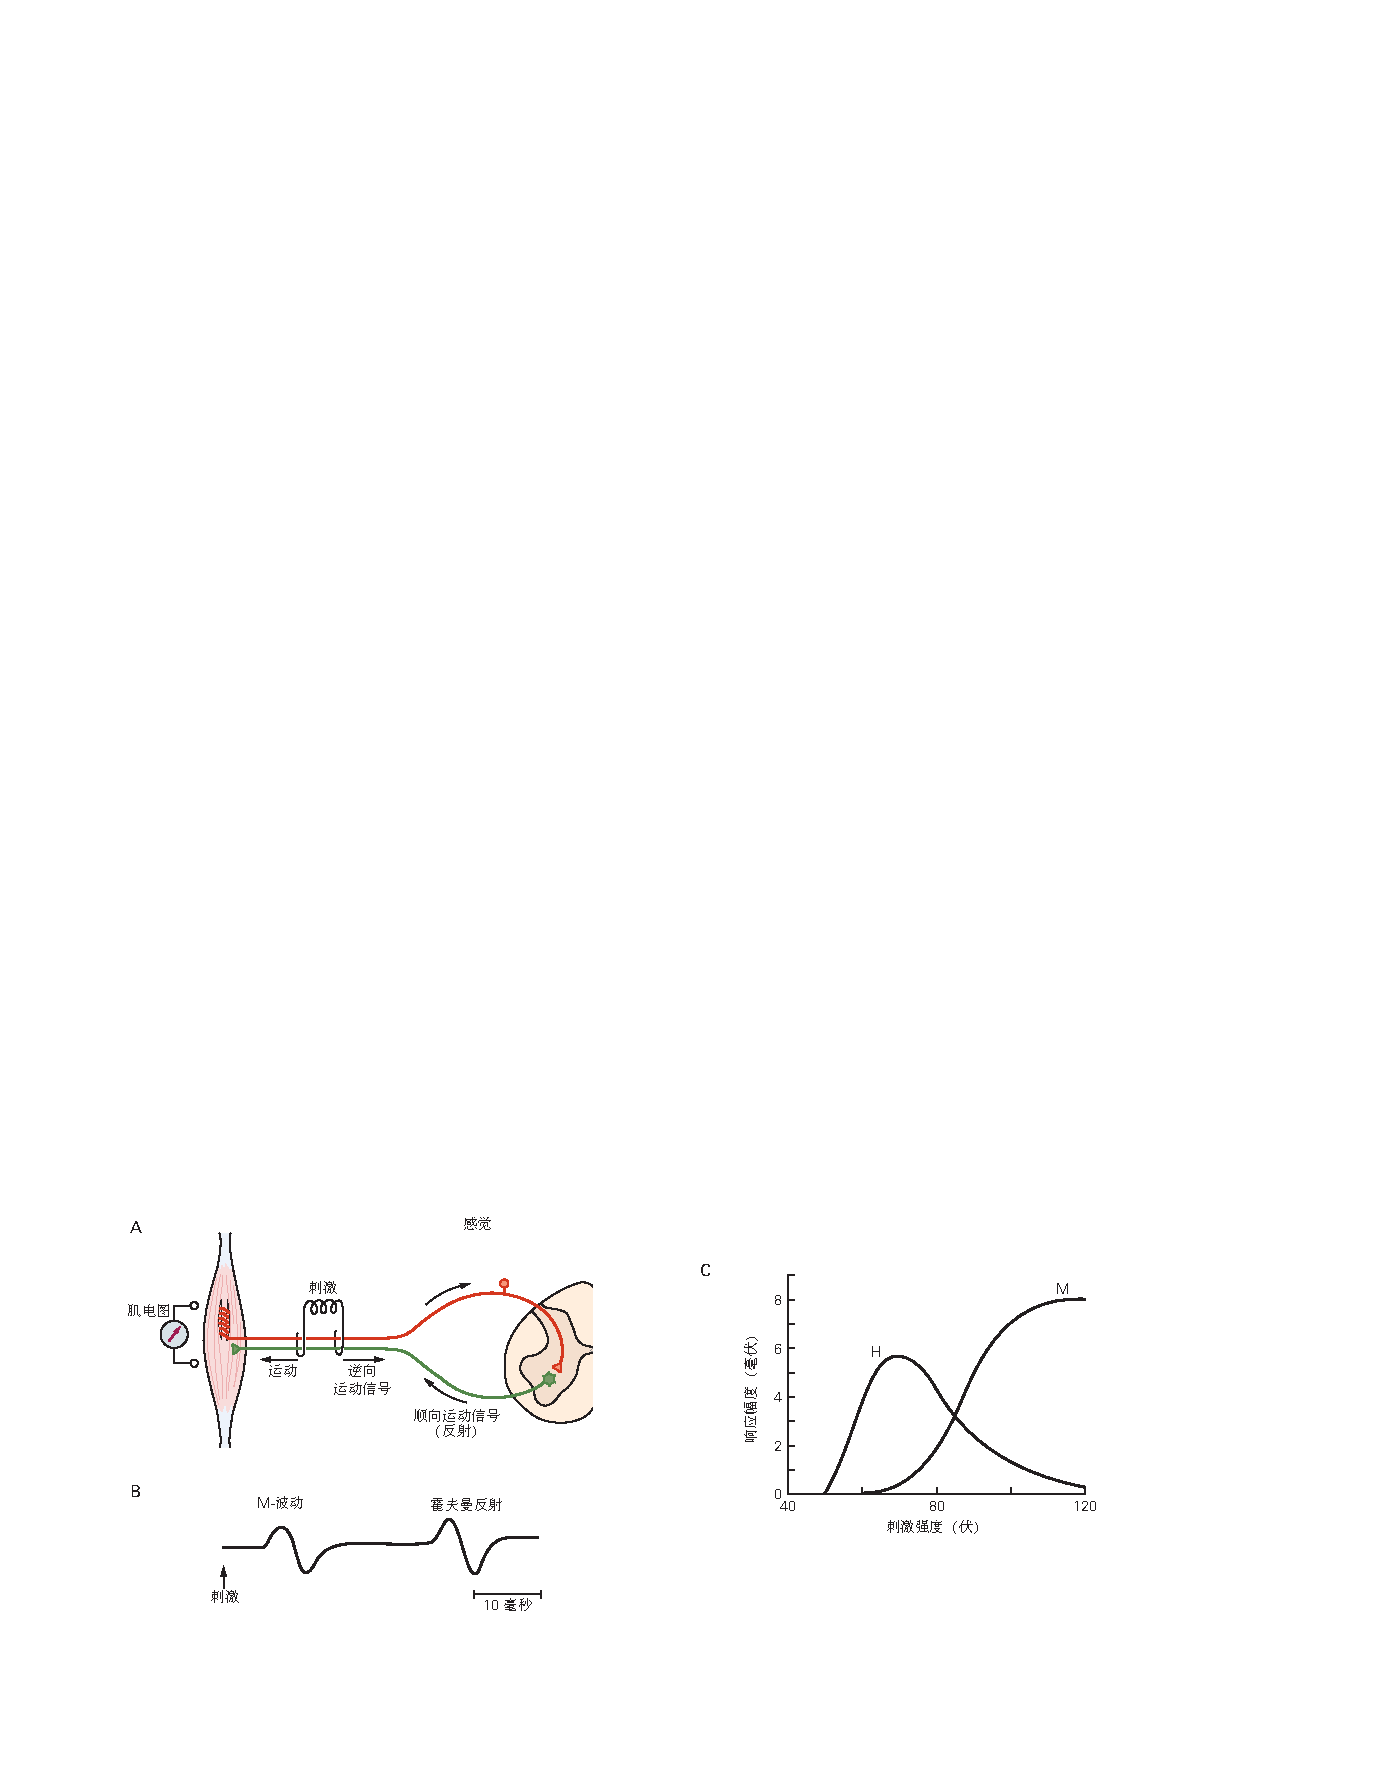
\includegraphics[width=1.0\linewidth]{chap32/fig_32_4}
	\caption{霍夫曼反射。
		\textbf{A.} 霍夫曼反射(H反射)是通过电刺激肌梭的\textit{大直径}感觉纤维而引起的。
		感觉纤维刺激$\alpha$运动神经元,进而激活肌肉。
		当使用混合神经时,运动神经元轴突也可以被直接激活。
		\textbf{B.} 在中等刺激强度下,肌电图中M波先于H波(H反射)。
		\textbf{C.} 随着刺激强度的增加,由纺锤体感觉纤维反射性产生的顺向性运动神经元尖峰被相同运动轴突中的电刺激引发的反向性尖峰所消除。}
	\label{fig:32_4}
\end{figure}


\textit{大直径}纤维与运动神经元的连接模式可以通过细胞内记录直接显示。
来自特定肌肉的\textit{大直径}纤维不仅会刺激支配同一(同名)肌肉的运动神经元,还会刺激支配具有类似机械作用的其他(异名)肌肉的运动神经元。


\textit{洛恩$\cdot$孟德尔}和\textit{埃尔伍德$\cdot$亨尼曼}使用一种被称为尖峰触发平均的计算机增强技术来确定单个\textit{大直径}纤维中的动作电位传输到脊髓运动神经元群的程度。
他们发现单个\textit{大直径}轴突与支配猫内侧腓肠肌的所有同名运动神经元形成兴奋性突触。
这种广泛的分歧有效地放大了单个\textit{大直径}纤维的信号,导致对它们起源的肌肉产生强烈的兴奋性驱动(自源性兴奋)。


反射通路中的\textit{大直径}轴突也为许多支配协同肌的运动神经元提供兴奋性输入(一些协同肌的运动神经元高达 60\%)(图~\ref{fig:32_1}A)。 
尽管广泛存在,但这些联系不如与同名运动神经元的联系牢固。


\begin{figure}[htbp]
	\centering
	\includegraphics[width=0.91\linewidth]{chap32/fig_32_1}
	\caption{脊髓反射涉及四肢众多肌肉的协调收缩。
		% 翘脚(膝跳反射)
		\textbf{A.} 在单突触通路中,来自肌梭的\textit{大直径}感觉轴突在两组运动神经元上建立兴奋性连接:支配它们产生的相同(同源)肌肉的$ \alpha $运动神经元和支配协同肌的运动神经元。 
		它们还通过中间神经元抑制支配\textit{拮抗肌}的运动神经元。
		当用反射锤敲击肌腱拉伸肌肉时,来自\textit{纺锤体}的感觉纤维的激活率会增加。
		这导致同一块肌肉及其\textit{协同肌}的收缩和\textit{拮抗肌}的松弛。
		因此,反射倾向于抵消拉伸,增强肌肉的弹簧状特性。
		右边的记录展示了一只去大脑猫的肌肉伸展所产生的收缩的反射性质。
		当伸肌被拉伸时,它通常会产生很大的力,但在\textit{背根}的感觉传入神经被切断后,它会产生非常小的力(虚线)\cite{liddell1924reflexes}。
		% 弯腿、伸腿
		\textbf{B.} 在多突触通路中,一条兴奋通路激活支配同侧\textit{屈肌}的运动神经元,使肢体远离有害刺激,而另一条通路同时激发支配\textit{对侧伸肌}的运动神经元,在撤回肢体时提供支撑。
		\textit{抑制性中间神经元}确保在反射反应期间供应拮抗肌的运动神经元不活跃\cite{schmidt1989motor}。}
	\label{fig:32_1}
\end{figure}


\textit{大直径}纤维还通过\textit{大直径}抑制性中间神经元向支配拮抗肌的 $ \alpha $ 运动神经元发送抑制信号。
这种突触抑制通路是相互神经支配的基础:
当肌肉被拉伸时,它的拮抗肌就会放松。



\subsection{$ \gamma $运动神经元调节肌肉纺锤体的敏感性}

肌梭的活动可以通过改变$ \gamma $运动神经元的活动水平来调节,$ \gamma $运动神经元支配肌梭的梭内肌纤维(方框~\ref{box:32_1})。
$ \gamma $运动神经元的这种功能,通常被称为肌梭运动系统,可以通过在实验条件下选择性地刺激 $ \alpha $ 和$ \gamma $运动神经元来证明。


当仅刺激 $ \alpha $ 运动神经元时,来自肌梭的\textit{大直径}纤维的发射在肌肉收缩期间暂停,因为肌肉正在缩短并因此卸载(松弛)纺锤。
但是,如果$ \gamma $运动神经元与$ \alpha $运动神经元同时被激活,则停顿被消除。
$ \gamma $ 运动神经元对梭内纤维的收缩使纺锤体保持在张力下,从而将\textit{大直径}纤维的放电率保持在最佳范围内,以发出长度变化信号,无论肌肉的实际长度如何(图~\ref{fig:32_5})。 
这种 $ \alpha $-$ \gamma $ 共激活被用于许多随意运动,因为它稳定了肌梭的敏感性。


\begin{figure}[htbp]
	\centering
	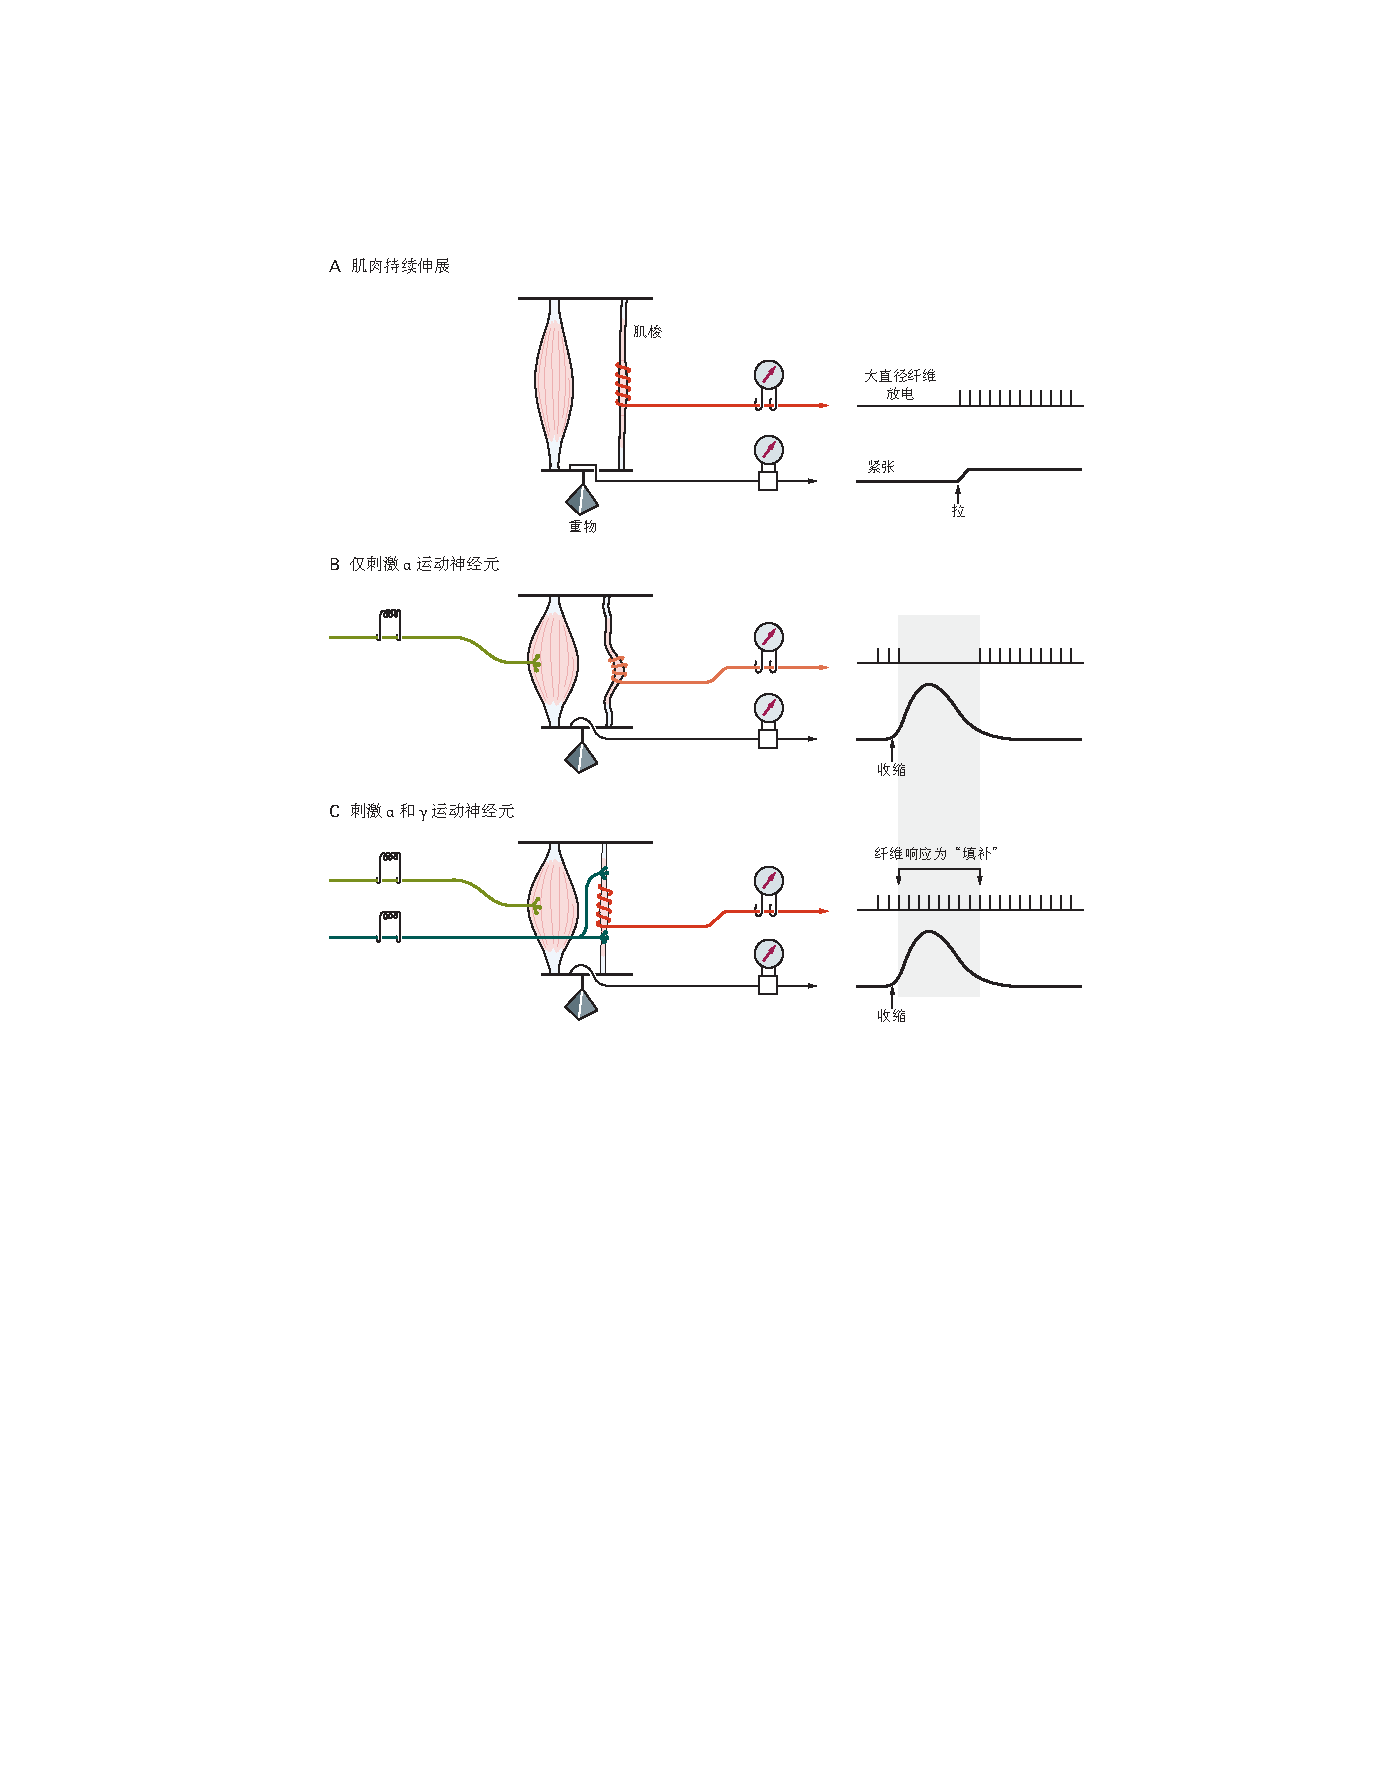
\includegraphics[width=0.92\linewidth]{chap32/fig_32_5}
	\caption{在主动肌肉收缩期间激活$ \gamma $运动神经元可维持肌梭对肌肉长度的敏感性\cite{hunt1951stretch}。
	\textbf{A.} 持续紧张会引起来自肌梭的\textit{大直径}感觉纤维稳定放电(两条肌纤维单独显示仅供说明)。
	\textbf{B.} 当 $ \alpha $ 运动神经元受到刺激时,\textit{大直径}纤维的放电会出现特征性停顿,导致肌肉短暂\textit{收缩}。
	\textit{大直径}纤维停止发射,因为纺锤体因收缩而卸载。
	\textbf{C.} $ \gamma $运动神经元支配肌梭梭内纤维的收缩极区(见图~\ref{fig:32_2}A)。
	如果$ \gamma $运动神经元与$ \alpha $运动神经元同时受到刺激,则纺锤体在收缩期间不会卸载。
	结果,当仅刺激 $ \alpha $ 运动神经元时发生的\textit{大直径}感觉纤维放电暂停被纤维对刺激$ \gamma $运动神经元的反应“填补”。}
	\label{fig:32_5}
\end{figure}


除了$ \gamma $运动神经元的轴突外,$ \alpha $ 运动神经元轴突的侧枝有时也会支配梭内纤维。
支配梭内和梭外肌纤维的轴突被称为$\beta$轴突。
$ \beta $ 轴突侧枝提供相当于 $ \alpha $-$ \gamma $ 共激活。
纺锤体中的 $ \beta $ 神经支配在猫和人类中都存在,尽管对于大多数肌肉来说它是无法量化的。


$ \beta $ 梭运动系统强制连接梭外和梭内收缩,突出了独立梭运动系统($ \gamma $运动神经元)的重要性。
事实上,在两栖动物等低等脊椎动物中,$ \beta $ 传出神经是梭内神经支配的唯一来源。
哺乳动物已经进化出一种机制,使肌梭不再完全依赖于它们母体肌肉的行为。
原则上,这种解耦可以更灵活地控制不同类型运动任务的主轴灵敏度。


在猫的各种自然运动过程中,纺锤体感觉轴突的记录支持了这一结论。
$ \gamma $运动神经元的活动量和类型设置在稳定水平,根据具体任务或环境而变化。
一般来说,随着运动速度和难度的增加,静态和动态$ \gamma $运动神经元(图~\ref{fig:32_2}B)的活动水平逐渐提高。
不可预测的情况,例如当猫被抱起或被抚摸时,会导致动态$ \gamma $运动神经元的活动显著增加,从而在肌肉拉伸时增加纺锤体反应。 
当动物执行一项艰巨的任务时,例如穿过狭窄的光束,静态和动态$ \gamma $激活都处于高水平(图~\ref{fig:32_6})。


\begin{figure}[htbp]
	\centering
	\includegraphics[width=1.0\linewidth]{chap32/fig_32_6}
	\caption{在主动肌肉收缩期间激活$ \gamma $运动神经元可维持肌梭对肌肉长度的敏感性\cite{hunt1951stretch}。 
	\textbf{A.} 持续紧张会引起来自肌梭的\textit{大直径}感觉纤维稳定放电(两条肌纤维单独显示仅供说明)。
	\textbf{B.} 当 $ \alpha $ 运动神经元受到刺激时,\textit{大直径}纤维的放电会出现特征性停顿,导致肌肉短暂收缩。
	\textit{大直径}纤维停止发射,因为纺锤体因收缩而卸载。
	\textbf{C.} $ \gamma $运动神经元支配肌梭梭内纤维的收缩极区(见图~\ref{fig:32_2}A)。
	如果$ \gamma $运动神经元与阿尔法运动神经元同时受到刺激,则纺锤体在收缩期间不会卸载。
	结果,当仅刺激 $ \alpha $ 运动神经元时发生的\textit{大直径}感觉纤维放电暂停被纤维对刺激$ \gamma $运动神经元的反应“填补”。}
	\label{fig:32_6}
\end{figure}


\begin{figure}[htbp]
	\centering
	\includegraphics[width=1.0\linewidth]{chap32/fig_32_2}
	\caption{肌梭检测肌肉长度的变化。
	\textbf{A}. 肌梭的主要成分是梭内肌纤维、感觉轴突末梢和运动轴突末梢。
	梭内纤维是特殊的肌肉纤维,中央区域不可收缩。
	$ \gamma $运动神经元支配梭内纤维的收缩极区。
	两极区域的收缩从两端拉动梭内纤维的中央区域。
	感觉末梢围绕梭内纤维的中央区域盘旋,并对这些纤维的拉伸做出反应\cite{hulliger1984mammalian}。
	\textbf{B}. 肌梭包含三种类型的梭内纤维:\textit{动态核袋纤维}、\textit{静态核袋纤维}和\textit{核链纤维}。
	单个\textit{大直径}感觉轴突支配所有三种类型的纤维,形成初级感觉末端。
	II 型感觉轴突支配核链纤维和静袋纤维,形成次级感觉末端。
	两种类型的运动神经元支配不同的梭内纤维。
	动态$ \gamma $运动神经元仅支配动态袋纤维;
	静态$ \gamma $运动神经元支配链状和静态袋状纤维的各种组合\cite{boyd1980isolated}。
	\textbf{C}. 两种类型的$ \gamma $运动神经元的选择性刺激对来自纺锤体的\textit{大直径}感觉纤维的放电有不同的影响。
	在没有$ \gamma $刺激的情况下,\textit{大直径}纤维显示出对肌肉拉伸的小动态响应和稳态放电的适度增加。
	当静态$ \gamma $运动神经元受到刺激时,\textit{大直径}纤维的稳态响应会增加,但动态响应会降低。
	当刺激动态$ \gamma $运动神经元时,\textit{大直径}纤维的动态反应明显增强,但稳态反应逐渐恢复到原来的水平\cite{brown1966subdivision}。}
	\label{fig:32_2}
\end{figure}


因此,神经系统使用梭运动系统微调肌梭,从而使肌梭的整体输出提供最适合任务的信息。
人类对 $ \alpha $ 和 $ \gamma $ 运动神经元进行独立控制的任务条件尚未明确确定。



\subsection{牵张反射还涉及多突触通路}

单突触\textit{大直径}通路并不是肌肉拉伸时激活的唯一脊髓反射通路。
来自肌梭的 II 型感觉纤维也被激活。
这些放电依赖于肌肉长度和$ \gamma $运动神经元活动(方框~\ref{box:32_1}),并连接到脊髓中不同数量的兴奋性和抑制性中间神经元。


一些中间神经元直接投射到脊髓运动神经元,而另一些则有更多的间接连接。
由于 II 型感觉纤维的传导速度较慢,信号通过中间神经元传递,与单突触牵张反射相比,II 型纤维引起的肌肉反应更小、更易变且延迟。
一些由 II 组纤维激活的中间神经元发送轴突穿过脊髓中线并引起交叉反射。
这种跨越中线的连接对于协调功能性运动任务中的双侧肌肉活动很重要。



\subsection{高尔基肌腱器官向脊髓提供力敏感反馈}

在被动动物中刺激高尔基肌腱器官或其 Ib 感觉纤维会产生同源运动神经元的突触抑制(自生抑制)和拮抗运动神经元的兴奋(相互激发)。
因此,这些效果与肌肉拉伸或刺激\textit{大直径}感觉轴突引起的反应完全相反。


这种自生抑制是由 Ib 抑制性中间神经元介导的。
这些抑制性中间神经元从高尔基肌腱器官接收它们的主要输入,高尔基肌腱器官是肌肉中发出张力信号的感觉受体(方框~\ref{box:32_4}),并且它们与同名运动神经元建立抑制性连接。
然而,活跃动物的肌腱器官对 Ib 感觉纤维的刺激并不总是抑制同源运动神经元。
事实上,正如我们稍后将看到的,在某些情况下刺激肌腱器官可能会激发同源运动神经元。


\begin{proposition}[神经解剖学导航术语] \label{box:32_4}
	
	\quad \quad 高尔基肌腱器官是细长的包裹结构,长约1毫米,直径 0.1 毫米,位于骨骼肌纤维和肌腱之间的交界处。
	每个胶囊包含几个编织的胶原纤维,这些胶原纤维串联到一组肌纤维上。
	
	\quad \quad 每个肌腱器官由单个Ib轴突支配,该轴突分支成囊内的许多细末端;
	这些末端与胶原束交织在一起(图~\ref{fig:32_7}A)。
	
	\quad \quad 肌腱器官的拉伸会拉直胶原纤维,从而压缩Ib神经末梢并使其发火。
	由于神经末梢与胶原纤维的联系如此紧密,即使是很小的肌腱拉伸也会压迫神经末梢。
	
	\quad \quad 肌梭对肌肉长度的变化最敏感,而肌腱器官对肌肉张力的变化最敏感。
	与含有受体的胶原纤维束相连的肌纤维的收缩是对肌腱器官的特别有效的刺激。
	因此,肌腱器官在正常运动过程中很容易被激活。
	人类自愿手指运动和正常行走的猫的单个Ib轴突记录证明了这一点。
	
	\quad \quad 对麻醉动物制剂的研究表明,肌肉中肌腱器官群体的平均活动水平是收缩肌肉总力量的良好指标(图~\ref{fig:32_7}B)。
	射击频率和力量之间的这种密切一致与肌腱器官不断测量收缩肌肉中的力量的观点是一致的。
	
\end{proposition}


\begin{figure}[htbp]
	\centering
	\includegraphics[width=1.0\linewidth]{chap32/fig_32_7}
	\caption{\textbf{A}. 当高尔基肌腱器官被拉伸(通常是由于肌肉收缩)时,Ib \textit{传入轴突}被\textit{胶原纤维}压缩(见放大),其放电速率增加\cite{biederman2013human}。
	\textbf{B.} 高尔基肌腱器官群的放电率是肌肉力量的信号。
	线性回归线显示了猫比目鱼肌高尔基肌腱器官的放电率和力之间的关系\cite{crago1982sampling}。}
	\label{fig:32_7}
\end{figure}


来自肌腱器官的感觉轴突的反射作用在自然情况下是复杂的,其中一个原因是 Ib 抑制性中间神经元也接收来自肌梭、皮肤受体和关节受体的输入(图~\ref{fig:32_8}A)。
此外,它们还接收来自各种下行通路的兴奋性和抑制性输入。


\begin{figure}[htbp]
	\centering
	\includegraphics[width=1.0\linewidth]{chap32/fig_32_8}
	\caption{来自高尔基肌腱器官的 Ib 感觉纤维的反射作用在运动过程中受到调节。
	\textbf{A}. Ib 抑制性中间神经元接收来自肌腱器官、肌梭(未显示)、关节和皮肤受体以及下行通路的输入。
	\textbf{B}. 当开始行走时,Ib 感觉纤维对伸肌运动神经元的作用从抑制逆转为兴奋。
	当动物休息时,来自踝伸肌的 Ib 纤维的刺激通过 Ib 抑制性中间神经元抑制踝伸肌运动神经元,如记录中的超极化所示。
	在行走过程中,Ib 抑制性中间神经元被抑制,而从 Ib 感觉纤维接收输入的兴奋性中间神经元受到行走指令系统的促进,从而打开从高尔基肌腱器官到运动神经元的 Ib 兴奋通路。}
	\label{fig:32_8}
\end{figure}


高尔基肌腱器官最初被认为具有保护功能,可防止肌肉受损。
假设它们总是抑制同名运动神经元,并且它们仅在肌肉紧张时才会放电。
我们现在知道,这些受体会发出肌肉张力的微小变化信号,从而为神经系统提供有关肌肉收缩状态的精确信息。


从肌腱器官、皮肤感受器和关节感受器到 Ib 抑制性中间神经元的会聚感觉输入(图~\ref{fig:32_8}A)可能允许在诸如抓取精致物体等活动中精确控制肌肉力量的脊柱。
当手到达物体时,来自皮肤受体的额外输入可能会促进 Ib 抑制性中间神经元的活动,从而降低肌肉收缩水平并允许轻柔地抓握。


与来自肌梭的\textit{大直径}纤维一样,来自肌腱器官的 Ib 纤维与运动神经元形成广泛的联系,运动神经元支配作用于不同关节的肌肉。
因此,来自肌腱器官的感觉纤维与 Ib 抑制性中间神经元的连接是调节整个肢体运动的脊髓网络的一部分。



\subsection{皮肤反射产生复杂的运动,起到保护和姿势功能的作用}

大多数反射通路涉及中间神经,其中一种反射途径是屈曲-缩回反射,在这种反射中,肢体会迅速从疼痛刺激中缩回。
屈曲收缩是一种保护性反射,其中离散刺激使该肢体中的所有屈肌协调收缩。
我们知道这是一种脊髓反射,因为它在脊髓完全横断后仍然存在。


屈曲-缩回反射的感觉信号激活不同的多突触反射通路。 
一种刺激支配受刺激肢体屈肌的运动神经元,而另一种抑制支配肢体伸肌的运动神经元(图~\ref{fig:32_1}B)。
这种反射可在对侧肢体产生相反的作用,即伸肌运动神经元的兴奋和屈肌运动神经元的抑制。
这种交叉伸展反射用于在脚从疼痛刺激中撤回期间增强姿势支撑。
激活另一条腿的伸肌可以抵消因抬起受刺激的肢体而增加的负荷。
因此,屈曲收缩是一个完整的、虽然简单的运动动作。


虽然屈曲反射相对刻板,但空间范围和肌肉收缩的力量都取决于刺激强度。
接触微热的炉子可能只会在手腕和肘部产生适度的快速缩回,而接触非常热的炉子总是会导致所有关节用力收缩,导致整个肢体快速缩回。
反射的持续时间通常随着刺激强度的增加而增加,并且屈曲反射产生的收缩总是比刺激更持久。


由于屈曲-缩回反射与踏步的相似性,人们一度认为屈曲反射在行走过程中产生屈肌收缩很重要。
然而,我们现在知道,步行神经控制系统的一个主要组成部分是一组不需要感觉刺激的内在脊髓回路(第~\ref{chap:chap33}~章)。
然而,在哺乳动物中,控制行走的内在脊髓回路共享许多参与屈曲反射的中间神经元。



\subsection{中间神经元上感觉输入的收敛增加了反射对运动的贡献的灵活性}

Ib 抑制性中间神经元不是唯一从许多不同感觉方式接收会聚输入的中间神经元。
大量不同的感觉信息汇聚在脊髓的中间神经元上,使它们能够整合来自肌肉、关节和皮肤的信息。


由 I 组和 II 组感觉纤维激活的中间神经元受到了特别关注。
一段时间以来,人们认为由 II 组纤维激活的兴奋性和抑制性中间神经元可以与由 Ib 组传入神经激活的中间神经元区分开来,但现在认为必须放弃这种区别,并且 I 组和 II 组纤维集中在普通人群中整合来自活动肌肉的力和长度信息的中间神经元,从而根据肌肉的长度、活动水平和外部负荷帮助协调肌肉活动。



\section{感觉反馈和下行运动命令在共同的脊髓神经元相互作用以产生自主运动}

正如\textit{迈克尔$\cdot$福斯特}在他 1879 年的生理学教科书中指出的那样,意志应该利用脊髓中的网络来产生协调的运动,“而不是求助于自己的类似器官”,这一定是一种“对身体的节约”。
随后 140 年的研究证实了这一猜想。


第一个证据来自对感觉纤维和下行通路的联合和单独刺激在猫脊髓运动神经元中引发的突触电位的细胞内记录。
当单独的刺激强度降低到刚好低于诱发突触电位的阈值时,以适当的间隔组合刺激会使突触电位重新出现。
这提供了感觉纤维和下行通路会聚到反射通路中常见中间神经元的证据(参见图~\ref{fig:13_14})。
来自脊髓中间神经元的直接记录证实了这一点,人类受试者的无创霍夫曼反射测试也证实了这一点(图~\ref{fig:32_9})。


\begin{figure}[htbp]
	\centering
	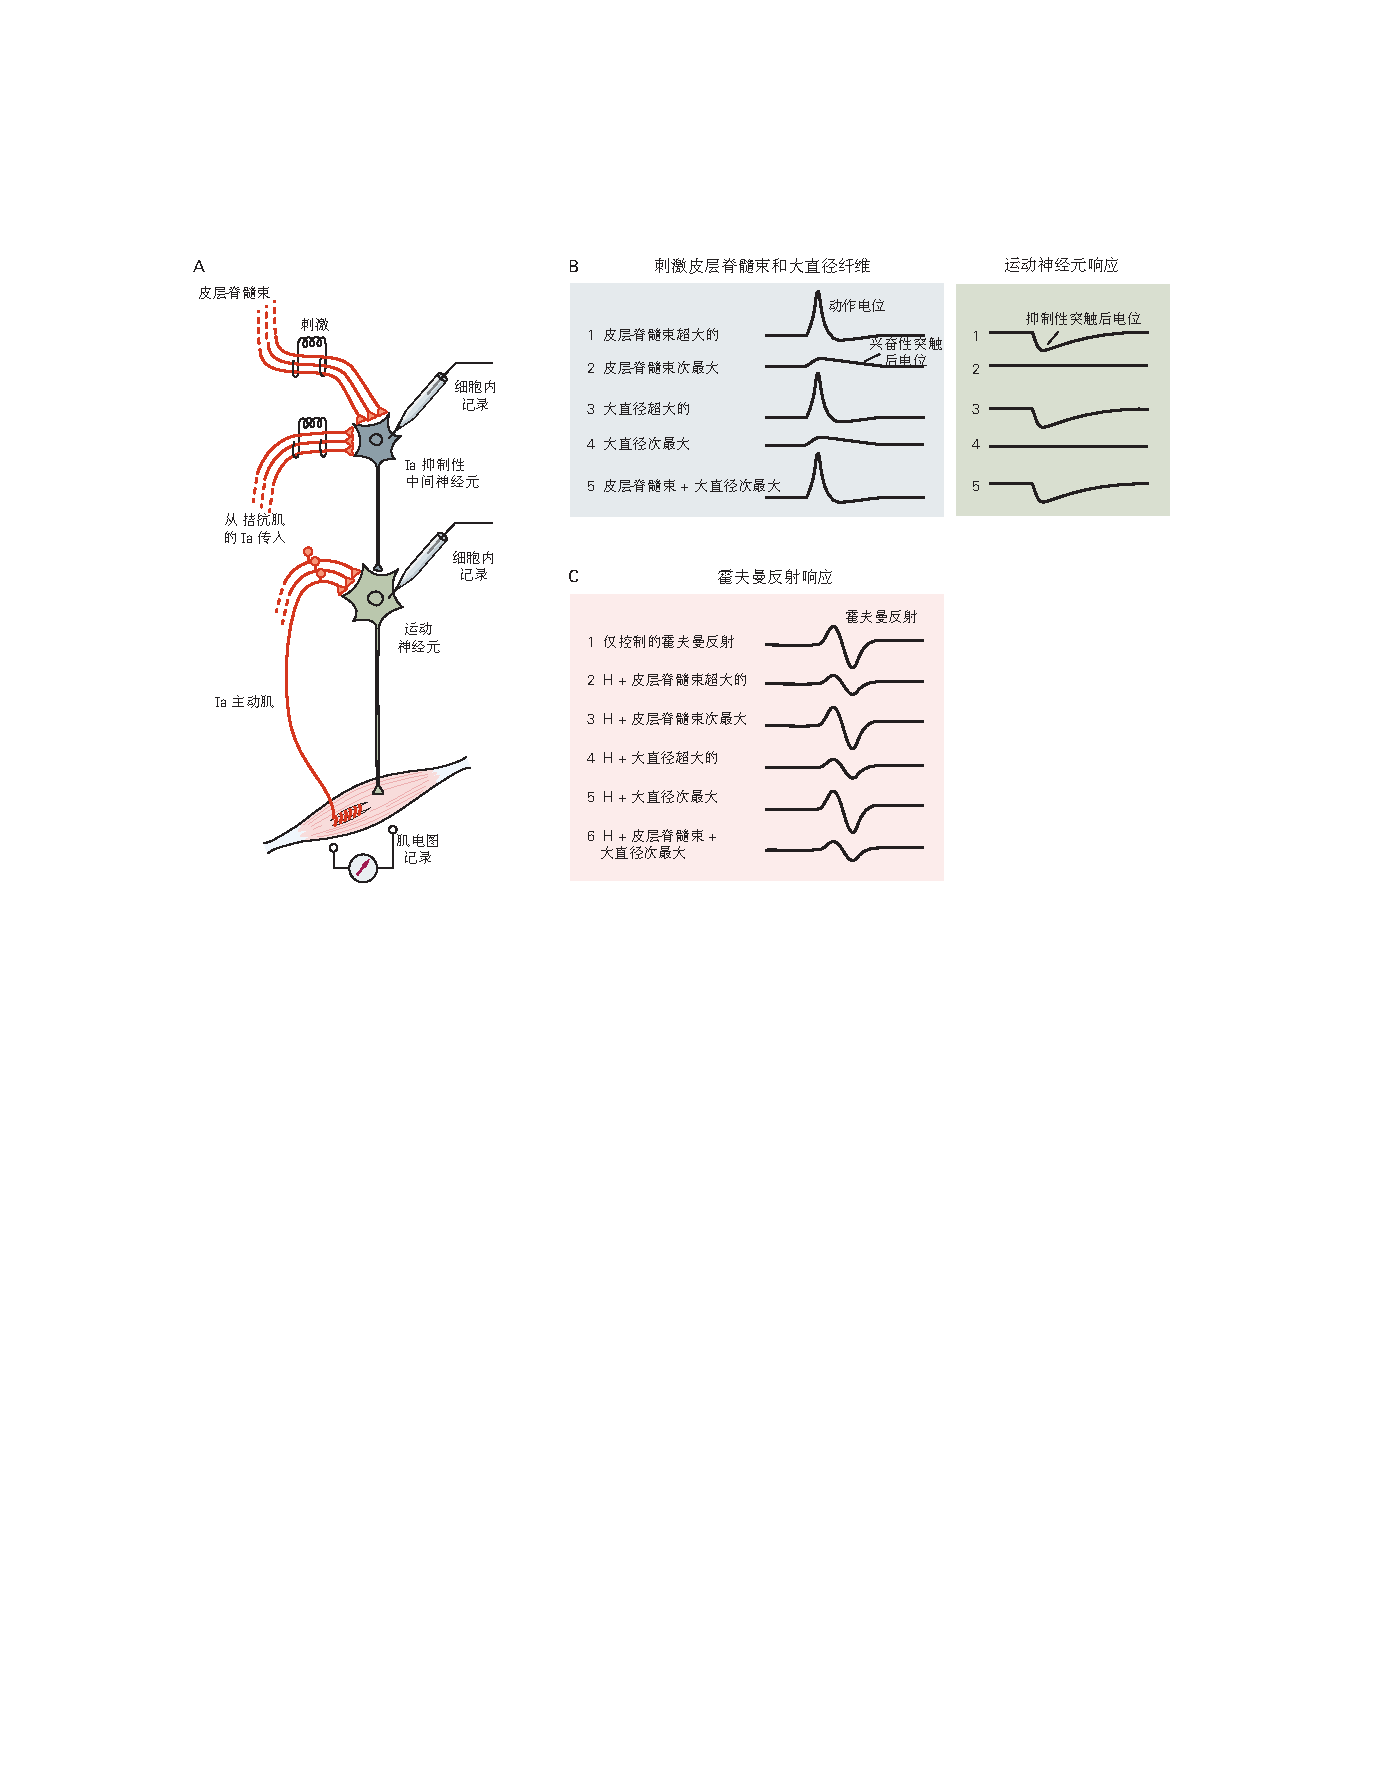
\includegraphics[width=1.0\linewidth]{chap32/fig_32_9}
	\caption{空间求和技术演示了如何整合来自下行输入和脊柱网络的信号。
	这项技术最初是在 1950 年代为研究猫的脊柱回路而引入的,但它也是后来研究人类脊柱运动控制机制的基础。
	它依赖于突触输入的空间总和(参见图~\ref{fig:13_14}),如此处使用相互\textit{大直径}抑制通路和\textit{皮层脊髓束}所示。
	\textbf{A}. 该图显示了用于测试兴奋性相互\textit{大直径}和皮层脊髓通路收敛到脊髓中\textit{大直径}抑制性中间神经元的实验装置。
	\textbf{B}. 在猫脊髓的急性实验中,分别对皮层脊髓纤维束(1)和\textit{大直径}轴突(3)施加超大刺激;
	每个刺激都会在运动神经元中引起\textit{抑制性突触后电位}。
	接下来,将两种刺激的强度降低到次最大水平,此时每条通路都无法在运动神经元中引发\textit{抑制性突触后电位}(2, 4)。
	然后,当两组次最大刺激配对时,它们在运动神经元中引发\textit{抑制性突触后电位}(5),从而得出两个输入通路汇聚在相同中间神经元上的结论。
	这通过\textit{大直径}抑制性中间神经元的直接记录得到证实。
	\textbf{C}. 在人类中,从中间神经元和运动神经元直接进行细胞内记录是不可能的,但是记录 H 反射(方框~\ref{box:32_4},图~\ref{fig:32_4})和皮层脊髓束的经皮刺激已经提供了类似于收敛的间接证据 在猫身上得到证明(见 B 部分)。
	H 反射的\textit{肌电图}记录可衡量脊髓运动神经元的兴奋性(1)。
	当\textit{皮层脊髓束}和拮抗剂\textit{大直径}纤维在超大水平分别受到刺激时,H 反射振幅由于在运动神经元中引发的复合\textit{抑制性突触后电位}而减弱(2, 4)。
	接下来,减少对抑制性中间神经元的这两个兴奋性通路的刺激,直到单独的刺激都不会引起 H 反射振幅的降低(3, 5)。
	然后,对两个次最大刺激进行定时,以在抑制性中间神经元中产生同步亚阈值\textit{兴奋性突触后电位}(6)。
	由于此协议导致 H 反射抑制,因此可以得出结论,\textit{皮层脊髓束}和\textit{大直径}传入神经元会聚在相同的\textit{大直径}抑制性中间神经元上。}
	\label{fig:32_9}
\end{figure}


直接证据表明,感觉反馈有助于通过人类的脊髓反射网络形成自主运动指令,这些证据来自对长度和力敏感的传入神经的感觉活动突然减少或消失的实验。
这可以通过在自主收缩期间突然放松或缩短肌肉来完成。
随之而来的肌肉活动减少的短暂潜伏期只能通过直接促进肌肉活动的反射通路的感觉活动来解释。



\subsection{肌肉纺锤体感觉传入活动通过\textit{大直径}单突触反射通路强化运动的中央指令}

牵张反射通路可以在自主运动和保持姿势期间促进运动神经元的调节,因为它们形成闭合反馈回路。
例如,拉伸肌肉会增加纺锤体感觉传入神经的活动,从而导致肌肉收缩和随之而来的肌肉缩短。
肌肉缩短反过来导致纺锤体传入神经活动减少、肌肉收缩减少和肌肉延长。


因此,牵张反射环持续作用(系统的输出,肌肉长度的变化,成为输入)趋向于使肌肉接近期望或参考长度。
牵张反射通路是一种负反馈系统或伺服机制,因为它倾向于抵消或减少与调节变量参考值的偏差。


1963 年,\textit{拉格纳$\cdot$格拉尼特}提出,自主运动的参考值是由作用于 $ \alpha $ 和 $ \gamma $ 运动神经元的递减信号设定的。
$ \alpha $ 运动神经元的放电率被设置为产生所需的肌肉缩短,$ \gamma $ 运动神经元的放电率被设置为产生肌梭的梭内纤维的等效缩短。
如果整个肌肉的缩短小于任务所需的,比如当负荷大于预期时,感觉纤维会增加它们的放电率,因为收缩的梭内纤维被相对较大的长度拉伸(加载) 整个肌肉。
如果缩短超过必要的程度,感觉纤维会降低其发射率,因为梭内纤维相对松弛(无负荷)(图~\ref{fig:32_10}A)。


\begin{figure}[htbp]
	\centering
	\includegraphics[width=1.0\linewidth]{chap32/fig_32_10}
	\caption{$ \alpha $ 运动神经元和$ \gamma $运动神经元的共同激活。
	\textbf{A}. 皮层运动命令对 $ \alpha $ 和 $ \gamma $ 运动神经元的共同激活允许来自肌梭的反馈加强 $ \alpha $ 运动神经元的激活。
	运动过程中的任何干扰都会改变肌肉的长度,从而改变来自纺锤波的感觉纤维的活动。
	改变的主轴输入到 $ \alpha $ 运动神经元补偿了干扰。
	\textbf{B.} 在手指缓慢弯曲期间,纺锤体\textit{大直径}感觉纤维的放电率增加。
	这种增加取决于 $ \alpha $-$ \gamma $ 共激活。
	如果$ \gamma $运动神经元不活跃,则纺锤体会松弛,其放电率会随着肌肉缩短而降低\cite{vallbo1981basic}。}
	\label{fig:32_10}
\end{figure}


从理论上讲,这种机制可以允许神经系统产生给定距离的运动,而无需事先知道实际的负载或移动的重量。
然而,在实践中,牵张反射通路对运动神经元没有足够的控制来克服巨大的意外负荷。
如果我们考虑一下当我们试图提起一个我们认为是空的沉重手提箱时会发生什么,这一点就很明显了。
不会对超出预期的负载进行自动补偿。
相反,我们必须暂停一下以计划一个具有更大肌肉激活的新运动。


强有力的证据表明,$ \alpha $ 运动神经元和$ \gamma $ 运动神经元在人类自愿运动过程中被共同激活,这来自对来自肌梭的感觉纤维活动的直接测量。
在 1960 年代后期,\textit{亚克$\cdot$威尔波}和\textit{卡尔$\cdot$艾瑞克$\cdot$哈格巴斯}开发了显微神经造影术,这是一种从周围神经中最大的传入纤维进行记录的技术。
\textit{威尔波}后来发现,在手指缓慢运动期间,来自收缩肌肉纺锤体的\textit{大直径}纤维会增加其发射率,即使肌肉在收缩时会缩短(图~\ref{fig:32_10}B)。
发生这种情况是因为与纺锤体有直接兴奋性联系的$ \gamma $运动神经元与阿尔法运动神经元共同激活。


此外,当受试者试图以恒定速度进行缓慢运动时,\textit{大直径}纤维的发射反映了运动轨迹中速度的微小偏差(有时肌肉缩短得很快,有时则更慢)。
当屈曲速度瞬时增加时,纤维的发射率会降低,因为肌肉缩短得更快,因此对梭内纤维施加的张力较小。
当速度降低时,放电增加,因为肌肉缩短得更慢,因此,梭内纤维的相对张力增加。
神经系统可以使用此信息通过激发阿尔法运动神经元来补偿运动轨迹中的不规则性。



\subsection{通过下行输入调节\textit{大直径}抑制性中间神经元和\textit{闰绍细胞}协调关节肌肉活动}

交互神经支配不仅对牵张反射有用,而且对随意运动也有用。
在运动过程中,拮抗肌的放松可以提高速度和效率,因为作为原动机的肌肉不会对抗对立肌肉的收缩。


\textit{大直径}抑制性中间神经元接收来自运动皮层神经元轴突侧支的输入,这些侧支与脊髓运动神经元建立直接兴奋性连接。
这种组织特征简化了自主运动的控制,因为高级中枢不必向相对的肌肉发送单独的命令。


有时同时收缩原动力和拮抗剂是有利的。
这种共同收缩具有加强关节的作用,并且在精度和关节稳定性至关重要时最有用。
这种现象的一个例子是在接球之前肘部屈肌和伸肌的共同收缩。
\textit{大直径}抑制性中间神经元接收来自所有主要下行通路的兴奋性和抑制性信号(图~\ref{fig:32_11}A)。
通过改变对这些中间神经元的兴奋性和抑制性输入的平衡,脊髓上中枢可以调节肌肉的相互抑制并实现共同收缩,从而控制关节刚度的相对量以满足运动行为的要求。



\begin{figure}[htbp]
	\centering
	\includegraphics[width=0.86\linewidth]{chap32/fig_32_11}
	\caption{抑制性脊髓中间神经元协调反射动作。
	\textbf{A}. \textit{大直径}抑制性中间神经元通过与运动神经元的不同接触调节牵张反射回路中拮抗肌的收缩。
	此外,中间神经元接收来自皮层脊髓和其他下行通路的兴奋性和抑制性输入。
	这些脊髓上信号的平衡变化允许中间神经元协调关节处拮抗肌的共同收缩。
	\textbf{B}. \textit{闰绍细胞}对运动神经元产生周期性抑制。
	这些中间神经元被来自运动神经元的侧支兴奋并抑制这些相同的运动神经元。
	这种负反馈系统调节运动神经元的兴奋性并稳定放电率。
	\textit{闰绍细胞}还向协同运动神经元(未显示)和与拮抗运动神经元形成突触的\textit{大直径}抑制性中间神经元发送侧枝。
	因此,调节\textit{闰绍细胞}兴奋性的下行输入调节了控制关节周围运动的所有运动神经元的兴奋性。}
	\label{fig:32_11}
\end{figure}


脊髓运动神经元的活动也受另一类重要的抑制性中间神经元 \textit{闰绍细胞}的调节。
被运动神经元轴突的侧支兴奋并接收来自下行通路的显著突触输入,\textit{闰绍细胞}与多个运动神经元群产生抑制性突触连接,包括激发它们的运动神经元,以及\textit{大直径}抑制性中间神经元(图~\ref{fig:32_11}B)。
与运动神经元的连接形成负反馈系统,调节运动神经元的放电率,而与\textit{大直径}抑制性中间神经元的连接调节拮抗运动神经元的抑制强度,例如与拮抗剂的共同收缩有关。
从\textit{闰绍细胞}胞到不同运动核的投射分布也有助于肌肉活动在运动过程中在功能协同作用中得到协调。



\subsection{下行运动命令可能会促进或抑制反射通路中的传输}

正如我们所见,在静止的动物中,来自伸肌的 Ib 感觉纤维对同向运动神经元具有抑制作用。
在运动过程中,它们对相同的运动神经元产生兴奋作用,因为突触抑制通路中的传递被抑制(图~\ref{fig:32_8}B),同时促进了通过兴奋性中间神经元的传递。


这种称为状态依赖性反射逆转的现象说明了脊髓回路中的传输如何通过下行运动命令来调节以满足运动过程中不断变化的要求。
通过有利于通过负荷敏感的高尔基肌腱器官的兴奋性通路进行传输,下行运动命令确保来自活跃肌肉的反馈自动促进肌肉的激活,从而大大简化了脊髓上中枢的任务。


状态依赖性反射逆转也在人类中得到证实。
刺激足部的皮肤和肌肉传入神经会促进在摆动期早期抬起足部的肌肉,但在摆动期后期会抑制相同肌肉的活动。
这两种效果都具有良好的功能意义。
在摆动阶段的早期,来自足部的正反馈将有助于将脚抬过障碍物,而在摆动后期抑制相同的肌肉将有助于将脚快速降低到地面,以便可以使用相反的障碍物通过障碍物。



\subsection{下行输入通过改变初级感觉纤维的突触效率来调节脊髓的感觉输入}

在 1950 年代和 1960 年代初期,\textit{约翰$\cdot$卡鲁$\cdot$埃克尔斯}和他的合作者证明,当其他\textit{大直径}纤维受到刺激时,通过刺激\textit{大直径}感觉纤维在猫脊髓运动神经元中引发的单突触\textit{兴奋性突触后电位}会变小。
这导致在脊髓中发现了几组 \textit{$\gamma$-氨基丁酸} 能抑制性中间神经元,它们对初级感觉神经元施加突触前抑制(图~\ref{fig:32_12})。 
一些中间神经元主要抑制\textit{大直径}感觉轴突,而其他神经元主要抑制 Ib 轴突或皮肤的感觉纤维。


\begin{figure}[htbp]
	\centering
	\includegraphics[width=0.6\linewidth]{chap32/fig_32_12}
	\caption{通过降低突触前抑制输入选择性调节初级感觉轴突末端有助于产生协调的肢体运动。
		由\textit{下行输入}激活的\textit{抑制性中间神经元}(蓝色)可以具有突触前或突触后效应。
		一些释放抑制性神经递质 \textit{$ \gamma $-氨基丁酸}的中间神经元与初级感觉纤维形成轴突-轴突突触。
		主要抑制机制涉及激活突触前\textit{大直径}感觉轴突末端的 \textit{$ \gamma $-氨基丁酸} 能受体,导致末端去极化和递质释放减少。
		这种突触前抑制广泛分布于脊髓中。
		来自一个屈肌的\textit{大直径}感觉纤维的刺激可能引起对支配整个肢体肌肉的运动神经元的屈肌和伸肌\textit{大直径}轴突末端的突触前抑制。
		然而,存在几种不同的介导突触前抑制的中间神经元群体,这允许对与自主运动相关的突触前抑制进行非常具体的调节。
		因此,皮质脊髓束中感觉输入与下行运动命令的相互作用可能会降低\textit{大直径}轴突末梢对激动性运动神经元(例如胫前运动神经元)的突触前抑制,同时增加\textit{大直径}末梢对拮抗性运动神经元(例如 , \textit{比目鱼肌}运动神经元)。
		因此,突触前抑制的调节可以同时促进对激动运动神经元激活的感觉反馈,同时减少拮抗肌的拉伸会引起牵张反射从而抵消运动的风险。}
	\label{fig:32_12}
\end{figure}


负责感觉抑制的主要机制是当终端上的 \textit{$ \gamma $-氨基丁酸} 能受体被激活时,由内向 \ce{Cl-} 电流引起的初级终端去极化。
这种去极化使终端中的一些 \ce{Na+} 通道失活,因此到达突触的动作电位的大小减小。
这样做的效果是减少了感觉传入神经递质的释放。


当通过外周传入神经的刺激进行测试时,突触前抑制在脊髓中广泛存在并影响四肢所有肌肉的初级传入神经。
然而,与其他中间神经元类似,负责突触前抑制的神经元也受下行通路控制,这使得与运动相关的突触前抑制的调节更加集中。
\textit{大直径}轴突与作为运动一部分被激活的肌肉运动神经元的突触前抑制在运动开始时减少。
相反,\textit{大直径}轴突对连接到不活跃肌肉的运动神经元的突触前抑制作用增加。
这种选择性调节的一个例子是\textit{大直径}轴突在其与拮抗运动神经元的突触处的突触前抑制增加,这部分解释了在激动剂收缩开始时拮抗肌中牵张反射的减少。
通过这种方式,神经系统利用\textit{大直径}轴突的广泛连接性,使用突触前抑制来塑造\textit{大直径}传入网络中的活动,以促进特定肌肉的激活。


突触前抑制提供了一种机制,神经系统可以通过该机制减少运动命令预测的感觉反馈,同时允许意外反馈进入脊髓运动回路和神经系统的其余部分。
与此功能一致,在高度可预测的运动(例如步行和跑步)期间,肌梭对\textit{大直径}感觉轴突的突触前抑制通常会增加。


最后,突触前抑制可以通过防止过度的感觉反馈和相关的自我强化振荡活动来帮助稳定运动的执行。



\section{部分自主运动下行命令通过脊髓中间神经元传递}

在猫和大多数其他脊椎动物中,皮层脊髓束与脊髓运动神经元没有直接联系;
所有的下行命令都必须通过脊髓中间神经元传递,这些中间神经元也是反射通路的一部分。
人类和\textit{旧大陆猴}是仅有的皮层脊髓神经元与脊髓腹角的脊髓运动神经元直接相连的物种。
即使在这些物种中,有相当一部分皮质脊髓束纤维终止于脊髓中间神经元的中间核,而终止于运动神经元的皮质脊髓纤维也有与中间神经元突触相连的侧枝。
因此,在到达运动神经元之前,皮层脊髓束中每个下行运动指令的相当一部分必须通过脊髓中间神经元传递,并与感觉活动整合。



\subsection{C3-C4 节段的本体脊髓神经元调节上肢运动的部分皮层脊髓命令}

在 1970 年代,\textit{安德斯$\cdot$伦德伯格}和他的合作者证明,猫脊髓 C3-C4 脊髓节段中的一组神经元将其轴突发送到位于更尾端颈椎节段的\textit{运动神经元}(图~\ref{fig:32_13})。
由于 C3-C4 节段中的神经元投射到支配一系列控制不同关节的前肢肌肉的运动神经元,并接收来自整个前肢皮肤和肌肉的输入,因此它们被命名为本体脊髓神经元。
除了来自皮肤和肌肉传入的感觉输入外,C3-C4 本体脊髓神经元还被来自皮层脊髓束的侧枝激活,从而将运动皮层的突触间兴奋传递到脊髓运动神经元。


\begin{figure}[htbp]
	\centering
	\includegraphics[width=0.58\linewidth]{chap32/fig_32_13}
	\caption{脊髓 C3-C4 节段中的本体脊髓神经元介导部分下行运动命令传递给颈椎运动神经元。
		一些皮质脊髓纤维(绿色)将侧枝输送到 C3-C4 节段(蓝色)中的\textit{脊髓固有神经元}。
		这些 C3-C4 本体脊髓神经元投射到位于更多颈椎尾段的\textit{运动神经元}。
		它们还接收来自肌肉传入的兴奋性输入,并将侧枝传送到\textit{外侧网状核}。}
	\label{fig:32_13}
\end{figure}


瑞典的\textit{布鲁尔$\cdot$阿尔斯特马克}和日本的\textit{伊佐正}随后进行的实验证实,类似的脊髓固有神经元也存在于猴子脊髓的 C3-C4 节段中,并且参与调节至少部分伸手运动命令。
非侵入性实验还提供了人类脊髓中 C3-C4 本体脊髓神经元存在的间接证据。
随着猴子和人类直接单突触皮层运动连接的进化,通过这种非突触通路的皮层脊髓传递可能变得不那么重要了。


接收来自肌肉的 I 组和 II 组感觉轴突的输入的腰椎中间神经元也接收来自下行运动束的重要输入,并为脊髓运动神经元提供兴奋性投射。
因此,这些中间神经元将自主运动的部分间接运动命令传递给控制腿部肌肉的脊髓运动神经元,并且可能相当于颈脊髓中 C3-C4 本体脊髓神经元。



\subsection{脊髓反射通路中的神经元在运动前被激活}

脊髓反射通路中的突触传递可能会根据运动意图而发生变化,与运动无关。
来自活跃猴子的细胞内记录表明,进行运动的意图会改变脊髓中间神经元的活动并改变脊髓反射通路中的传递。
类似地,在被阻止肌肉收缩的人类受试者中(通过将利多卡因注射到供应肌肉的周围神经中),收缩肌肉的自愿努力仍然会改变反射通路中的传输,就好像运动确实发生了一样。


在人类和猴子中,脊髓中间神经元也会在实际运动之前就改变了它们的活动。
例如,在人类受试者中,在即将被激活的肌肉中引发的霍夫曼反射在收缩开始前 50 毫秒就被激活,并在整个运动过程中保持激活状态。
相反,拮抗肌的反射受到抑制。
在运动开始之前抑制拮抗肌中的牵张反射是防止拮抗肌在主动肌收缩开始时被拉伸时被反射性激活的有效方法。


脊髓反射通路中的传输也可以根据更高的认知功能进行修改。
两个例子是
(1) 想象踩下脚踏板的人类受试者的比目鱼肌肌腱反射的增加 
(2)当受试者分别观察抓握和行走运动时手臂和腿部肌肉的霍夫曼反射的调节。



\section{本体感受反射在调节自主运动和自动运动中起着重要作用}

所有运动都会激活肌肉、关节和皮肤中的感受器。
身体自身运动产生的感觉信号被\textit{谢林顿}称为本体感受,他提出它们控制着正常运动的重要方面。
一个很好的例子是\textit{黑-伯反射},它调节灵感的幅度。
肺部的牵张感受器在吸气时被激活,当肺部扩张时,\textit{黑-伯反射}反射最终触发肺部扩张时从吸气到呼气的转变。


许多动物的行走系统也存在类似情况;
接近站立阶段结束时产生的感觉信号启动了摆动阶段的开始(第~\ref{chap:chap33}~章)。
对手臂感觉神经病患者的研究中显示,本体感受信号也有助于调节自主运动期间的运动活动。
这些患者表现出异常的伸展动作,并且难以准确定位肢体,因为缺乏本体感觉导致无法补偿人类手臂的复杂惯性特性。


因此,本体感受反射在调节自主运动中的一个主要功能是根据身体和四肢的生物力学状态的变化来调整运动输出。
这种调整确保了运动过程中运动活动的协调模式,并补偿了运动输出的内在可变性。



\section{脊髓反射通路经历长时变化}

脊髓反射通路中的传输经过调制,不仅可以满足运动的即时要求,还可以使运动命令适应个人的运动体验。
例如,当受试者提高其协调激动剂和拮抗剂收缩的能力时,相互\textit{大直径}抑制途径中的传输显示出逐渐变化。
长时间卧床休息或固定不动后不活动也会导致牵张反射和 H 反射发生变化。
相反,训练有素的芭蕾舞演员的比目鱼肌牵张反射较低,并且在不同类型的运动员中有所不同。


\textit{乔纳森$\cdot$沃尔帕乌}和他的同事对人类、猴子和老鼠进行的广泛研究发现,牵张反射可以操作性地调节以增加或减少。
这些变化背后的机制很复杂,涉及多个部位的改变,包括运动神经元特性的变化。
这些变化的一般先决条件是脊髓运动回路的皮层脊髓控制必须完好无损。



\section{中枢神经系统的损伤会导致反射反应的特征性改变}

牵张反射通常用于神经系统疾病患者的临床检查。
它们通常是通过用反射锤猛烈敲击肌肉的肌腱而引出的。
尽管这些反应通常称为肌腱反射或肌腱反射,但受刺激的感受器肌梭实际上位于肌肉而非肌腱中。
只有纺锤体中的主要感觉纤维参与腱反射,因为这些纤维被腱拍产生的肌肉快速拉伸选择性地激活。


测量牵张反射强度的变化可以帮助诊断某些病症以及定位中枢神经系统的损伤或疾病。
牵张反射缺失或活动减退通常表明外周反射通路的一个或多个组成部分发生了紊乱:感觉或运动轴突、运动神经元的细胞体或肌肉本身(第~\ref{chap:chap57}~章)。
然而,由于运动神经元的兴奋性取决于下行的兴奋性和抑制性信号,因此中枢神经系统损伤也可能导致牵张反射缺失或活动减退。
相反,过度活跃的牵张反射总是表明病变位于中枢神经系统。



\subsection{脊髓下行通路中断经常导致痉挛}

肌肉抵抗拉长的力量取决于肌肉的内在弹性或刚度。
因为肌肉具有串联和并联的弹性元件来抵抗延长,所以它表现得像弹簧(第~\ref{chap:chap31}~章)。
此外,肌肉内部和周围的结缔组织也可能导致其僵硬。
这些弹性元件可能会在大脑和脊髓损伤后发生病理改变,从而导致挛缩和异常的关节位置。
然而,肌肉对拉伸的抵抗力也有神经作用;
牵张反射通路中固有的反馈回路起到抵抗肌肉拉长的作用。


痉挛的特征是过度活跃的肌腱抽搐和对肌肉快速拉伸的抵抗力增加。
关节的缓慢运动只会引起被动阻力,这是由关节、肌腱、肌肉和结缔组织的弹性特性引起的。
随着拉伸速度的增加,拉伸阻力逐渐增加。
这种相位关系是痉挛的特征;
主动反射收缩仅发生在快速拉伸期间,当肌肉保持在拉长位置时,反射收缩减弱。


中风、大脑或脊髓损伤以及多发性硬化症等退行性疾病引起的下行运动通路损伤后会出现痉挛。
它也见于出生前、出生时或出生后不久发生脑损伤的个体,导致脑瘫。


下行通路损伤后不会立即出现痉挛,而是会在数天、数周甚至数月后发展。
这与拉伸反射回路中多个位置的塑性变化相似。
感觉\textit{大直径}组轴突在活跃时会释放更多的递质物质,而 $ \alpha $ 运动神经元会改变其内在特性和形态(树突萌芽和去神经超敏反应),从而使它们变得更加兴奋。
投射到运动神经元的兴奋性和抑制性中间神经元也会发生变化,并且可能有助于增加兴奋性。


无论产生痉挛的确切机制是什么,其作用都是强烈促进单突触反射通路中的传递。
它不是唯一受下行运动通路损伤影响的反射通路。
涉及 I/II 组中间神经元和来自皮肤的感觉纤维的通路也受到影响,并表现出在中枢运动损伤患者中观察到的症状。
因此,在临床上,痉挛在更广泛的意义上使用,而不仅仅与牵张反射过度兴奋有关。
反射性过度兴奋是否会导致下行通路损伤后的运动障碍,或者它是否可能是一种相关的适应性,有助于在下行输入减少时激活肌肉,这仍然存在争议。



\subsection{人类脊髓损伤导致一段脊髓休克期,随后出现反射亢进}

脊髓损伤会引起脊髓反射强度的巨大变化。
每年,大约有 1 万 1 千名美国人遭受脊髓损伤,还有更多人患有中风。
这些伤害中有一半以上会导致永久性残疾,包括运动和感觉功能受损以及无法控制大小便。
今天在美国大约有 25 万人因脊髓损伤而导致永久性残疾。


当脊髓被完全横断时,通常在受伤后会立即出现一段时期,此时横断面以下的所有脊髓反射都会减弱或完全抑制,这种情况称为脊髓休克。
在数周和数月的过程中,脊髓反射逐渐恢复,而且常常被大大增强。
例如,轻触足部皮肤可能会引起腿部强烈的屈曲缩回。



\section{要点}

1. 反射是由外周受体受到刺激而引发的协调的、无意识的运动反应。


2. 脊髓反射通路中的许多中间神经元组也参与产生复杂的运动,例如行走和从大脑传递自愿命令。


3. 反射反应的某些组成部分,尤其是那些涉及四肢的反射反应,是由脊髓上中枢介导的,例如脑干核团、小脑和运动皮层。


4. 由于感觉信号会聚到参与启动运动的脊柱和脊柱上神经元间系统,因此反射被顺利地整合到中央生成的运动指令中。
确定这些综合事件的细节是当代脊髓感觉运动整合研究的主要挑战之一。


5. 由于脊髓上中枢在脊髓反射通路中的作用,中枢神经系统的损伤或疾病通常会导致脊髓反射强度的显著改变。
变化模式为神经系统疾病患者的诊断提供了重要帮助。
